\documentclass[pdf, 12pt]
{beamer}
\mode<presentation>{\usetheme{Warsaw}}

\usepackage{amsmath, amsthm, amssymb, amsfonts, latexsym, mathtools}
\usepackage{enumerate}
\usepackage{graphicx}
\usepackage{bm}
\usepackage{physics}
\usepackage{pgf,tikz}
\usepackage{mathrsfs}
\usetikzlibrary{arrows}

% Environments
\theoremstyle{definition}
\newtheorem{algorithm}{Algorithm}
\newtheorem*{main}{Main Theorem}
\newtheorem{proposition}{Proposition}
\theoremstyle{remark}
\newtheorem*{notation}{Notation}

% Commands and operators
\newcommand{\ind}{\hspace*{0.5cm}}
\newcommand{\gap}{\hspace*{0.25cm}}
\newcommand*{\Cdot}{\raisebox{-0.25ex}{\scalebox{1.3}{$\cdot$}}}
\newcommand{\vect}[1]{\mathbf{#1}}
\newcommand{\transpose}{T}
\DeclareMathOperator{\interior}{\textbf{int}}
\DeclareMathOperator{\domain}{\textbf{dom}}
\DeclareMathOperator{\diag}{\textbf{diag}}
\DeclareMathOperator{\sign}{\textbf{sign}}
\DeclareMathOperator{\CG}{\textbf{CG}}
\DeclareMathOperator{\vol}{\textbf{vol}}
\DeclareMathOperator{\CC}{\textbf{CC}}
\DeclareMathOperator{\AC}{\textbf{AC}}
\DeclareMathOperator{\centerr}{\textbf{center}}

%% preamble
\title[Cutting-plane methods]{Cutting-plane methods with applications in convex optimization and active learning}
\author{David Wu}
\date{}
\begin{document}

%% title frame
\begin{frame}
\titlepage
\end{frame}

%% normal frame
\begin{frame}{Structure}
    \begin{itemize}
        \item General cutting-plane algorithm
        \item Analytic center
        \item Solving an active learning problem
   \end{itemize}
\end{frame}

\begin{frame}{The generic problem}
      Given a bounded convex polyhedron $\mathcal{P}_0$ defined by linear inequalities $a_i^\transpose x \leq b, i = 1, \dots, m$ known to contain a target set $X$ how do we find a point in $X$? 
\end{frame}

\begin{frame}
    \begin{figure}
    \centering
    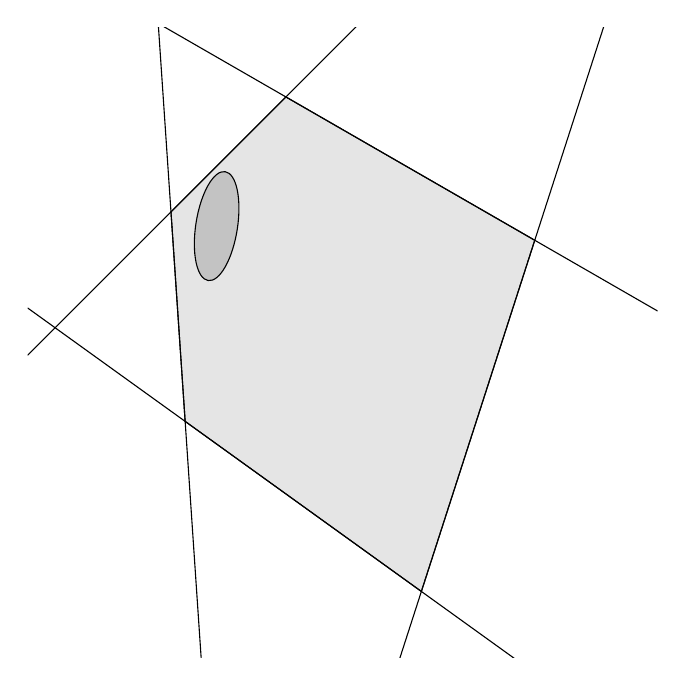
\begin{tikzpicture}[line cap=round,line join=round,>=triangle 45,x=1.0cm,y=1.0cm]
    \clip(-4.,-4.) rectangle (4.,4.);
    \fill[fill=black,fill opacity=0.1] (-2.18,1.66) -- (-2.,-1.) -- (1.,-3.16) -- (2.44,1.3) -- (-0.72,3.12) -- cycle;
    \draw [domain=-4.:4.] plot(\x,{(-5.6064-1.46*\x)/-1.46});
    \draw [domain=-4.:4.] plot(\x,{(-5.5-2.66*\x)/0.18});
    \draw [domain=-4.:4.] plot(\x,{(-7.32-2.16*\x)/3.});
    \draw [domain=-4.:4.] plot(\x,{(-9.0104--4.46*\x)/1.44});
    \draw [domain=-4.:4.] plot(\x,{(-8.5488--1.82*\x)/-3.16});
    \draw (-2.18,1.66)-- (-2.,-1.);
    \draw (-2.,-1.)-- (1.,-3.16);
    \draw (1.,-3.16)-- (2.44,1.3);
    \draw (2.44,1.3)-- (-0.72,3.12);
    \draw (-0.72,3.12)-- (-2.18,1.66);
    \draw [rotate around={81.1193408494798:(-1.6,1.48)},fill=black,fill opacity=0.15] (-1.6,1.48) ellipse (0.6998119774724771cm and 0.2648335398206404cm);
    \end{tikzpicture}  
    \end{figure}
\end{frame}

\begin{frame}[Strategy]
    \begin{itemize}
          \item Iterative approach
          \item Each iteration: 
          \begin{itemize}
                \item Choose a \emph{query point} $x$  
                \item Use $x$ and problem-specific information to \emph{construct} a cutting-plane, that is, to make a \emph{cut}
          \end{itemize}
          \item Repeat until a point in $X$ is found or stopping criterion is satisfied
    \end{itemize}
\end{frame}

\begin{frame}
    \begin{figure}
    \centering
    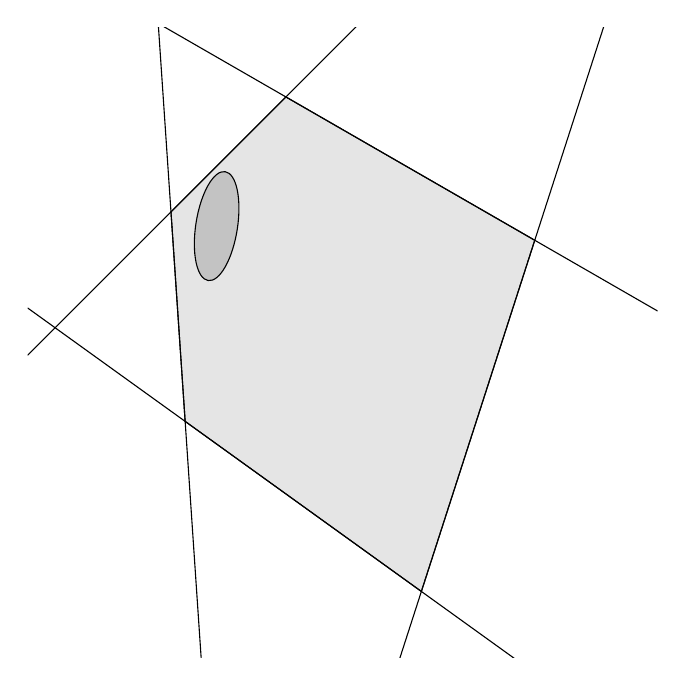
\begin{tikzpicture}[line cap=round,line join=round,>=triangle 45,x=1.0cm,y=1.0cm]
    \clip(-4.,-4.) rectangle (4.,4.);
    \fill[fill=black,fill opacity=0.1] (-2.18,1.66) -- (-2.,-1.) -- (1.,-3.16) -- (2.44,1.3) -- (-0.72,3.12) -- cycle;
    \draw [domain=-4.:4.] plot(\x,{(-5.6064-1.46*\x)/-1.46});
    \draw [domain=-4.:4.] plot(\x,{(-5.5-2.66*\x)/0.18});
    \draw [domain=-4.:4.] plot(\x,{(-7.32-2.16*\x)/3.});
    \draw [domain=-4.:4.] plot(\x,{(-9.0104--4.46*\x)/1.44});
    \draw [domain=-4.:4.] plot(\x,{(-8.5488--1.82*\x)/-3.16});
    \draw (-2.18,1.66)-- (-2.,-1.);
    \draw (-2.,-1.)-- (1.,-3.16);
    \draw (1.,-3.16)-- (2.44,1.3);
    \draw (2.44,1.3)-- (-0.72,3.12);
    \draw (-0.72,3.12)-- (-2.18,1.66);
    \draw [rotate around={81.1193408494798:(-1.6,1.48)},fill=black,fill opacity=0.15] (-1.6,1.48) ellipse (0.6998119774724771cm and 0.2648335398206404cm);
    \end{tikzpicture}  
    \end{figure}
\end{frame}

\begin{frame}
    \begin{figure}
    \centering
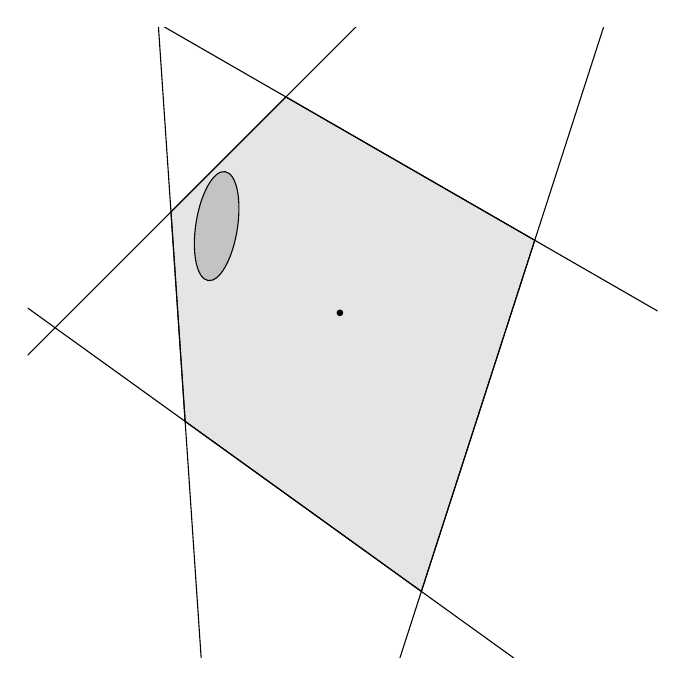
\begin{tikzpicture}[line cap=round,line join=round,>=triangle 45,x=1.0cm,y=1.0cm]
\clip(-4.,-4.) rectangle (4.,4.);
\fill[fill=black,fill opacity=0.1] (-2.18,1.66) -- (-2.,-1.) -- (1.,-3.16) -- (2.44,1.3) -- (-0.72,3.12) -- cycle;
\draw [domain=-4.:4.] plot(\x,{(-5.6064-1.46*\x)/-1.46});
\draw [domain=-4.:4.] plot(\x,{(-5.5-2.66*\x)/0.18});
\draw [domain=-4.:4.] plot(\x,{(-7.32-2.16*\x)/3.});
\draw [domain=-4.:4.] plot(\x,{(-9.0104--4.46*\x)/1.44});
\draw [domain=-4.:4.] plot(\x,{(-8.5488--1.82*\x)/-3.16});
\draw (-2.18,1.66)-- (-2.,-1.);
\draw (-2.,-1.)-- (1.,-3.16);
\draw (1.,-3.16)-- (2.44,1.3);
\draw (2.44,1.3)-- (-0.72,3.12);
\draw (-0.72,3.12)-- (-2.18,1.66);
\draw [rotate around={81.1193408494798:(-1.6,1.48)},fill=black,fill opacity=0.15] (-1.6,1.48) ellipse (0.6998119774724771cm and 0.2648335398206404cm);
\begin{scriptsize}
\draw [fill=black] (-0.034431088086562124,0.37895249068175696) circle (1.0pt);
\end{scriptsize}
\end{tikzpicture}    
    \end{figure}
\end{frame}

\begin{frame}
      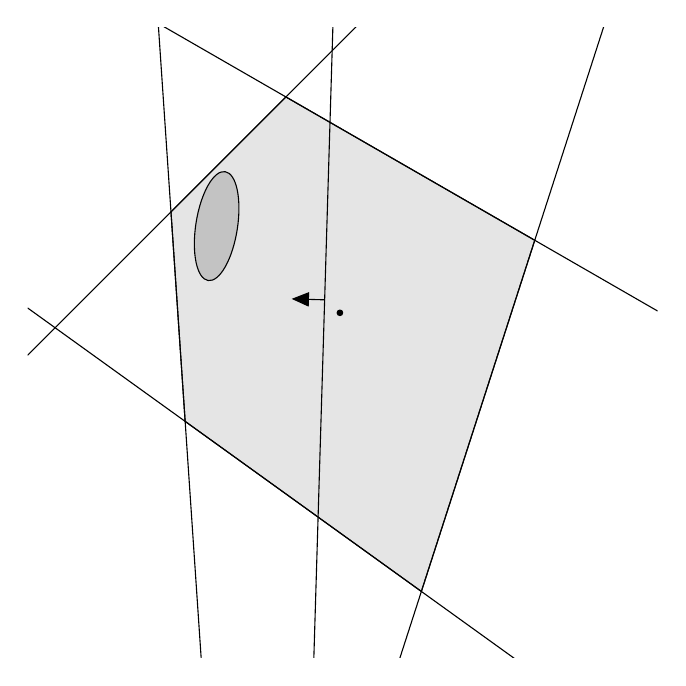
\begin{tikzpicture}[line cap=round,line join=round,>=triangle 45,x=1.0cm,y=1.0cm]
\clip(-4.,-4.) rectangle (4.,4.);
\fill[fill=black,fill opacity=0.1] (-2.18,1.66) -- (-2.,-1.) -- (1.,-3.16) -- (2.44,1.3) -- (-0.72,3.12) -- cycle;
\draw [domain=-4.:4.] plot(\x,{(-5.6064-1.46*\x)/-1.46});
\draw [domain=-4.:4.] plot(\x,{(-5.5-2.66*\x)/0.18});
\draw [domain=-4.:4.] plot(\x,{(-7.32-2.16*\x)/3.});
\draw [domain=-4.:4.] plot(\x,{(-9.0104--4.46*\x)/1.44});
\draw [domain=-4.:4.] plot(\x,{(-8.5488--1.82*\x)/-3.16});
\draw (-2.18,1.66)-- (-2.,-1.);
\draw (-2.,-1.)-- (1.,-3.16);
\draw (1.,-3.16)-- (2.44,1.3);
\draw (2.44,1.3)-- (-0.72,3.12);
\draw (-0.72,3.12)-- (-2.18,1.66);
\draw [rotate around={81.1193408494798:(-1.6,1.48)},fill=black,fill opacity=0.15] (-1.6,1.48) ellipse (0.6998119774724771cm and 0.2648335398206404cm);
\draw [domain=-4.:4.] plot(\x,{(-1.434464353569918-5.858898727052687*\x)/-0.1767771167645208});
\draw [->] (-0.2284304493558555,0.5436986776226944) -- (-0.6470492509991373,0.5556692684449995);
\begin{scriptsize}
\draw [fill=black] (-0.034431088086562124,0.37895249068175696) circle (1.0pt);
\end{scriptsize}
\end{tikzpicture}
\end{frame}

\begin{frame}
      \begin{figure}
            \centering 
            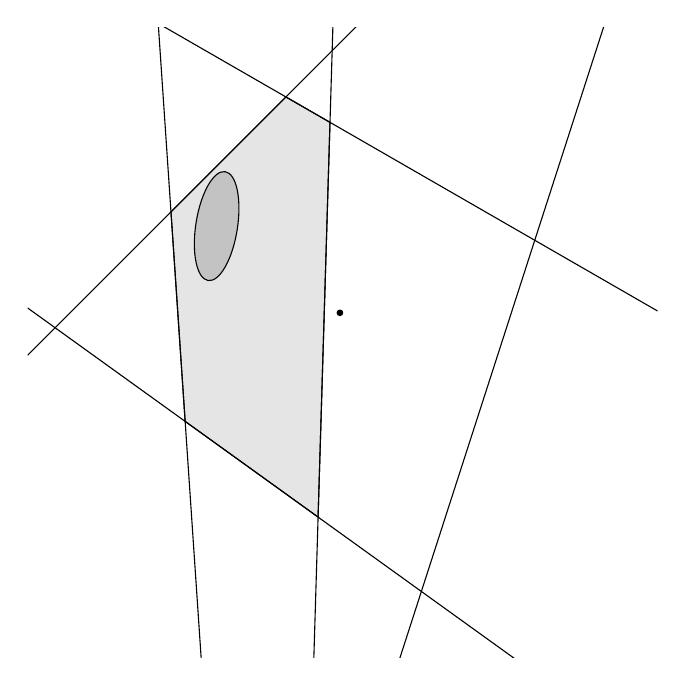
\begin{tikzpicture}[line cap=round,line join=round,>=triangle 45,x=1.0cm,y=1.0cm]
\clip(-4.,-4.) rectangle (4.,4.);
\fill[fill=black,fill opacity=0.1] (-2.,-1.) -- (-0.31168475782111604,-2.2155869743687964) -- (-0.16042145413452763,2.7977110906724176) -- (-0.72,3.12) -- (-2.18,1.66) -- cycle;
\draw [domain=-4.:4.] plot(\x,{(-5.6064-1.46*\x)/-1.46});
\draw [domain=-4.:4.] plot(\x,{(-5.5-2.66*\x)/0.18});
\draw [domain=-4.:4.] plot(\x,{(-7.32-2.16*\x)/3.});
\draw [domain=-4.:4.] plot(\x,{(-9.0104--4.46*\x)/1.44});
\draw [domain=-4.:4.] plot(\x,{(-8.5488--1.82*\x)/-3.16});
\draw [rotate around={81.1193408494798:(-1.6,1.48)},fill=black,fill opacity=0.15] (-1.6,1.48) ellipse (0.6998119774724771cm and 0.2648335398206404cm);
\draw [domain=-4.:4.] plot(\x,{(-1.434464353569918-5.858898727052687*\x)/-0.1767771167645208});
\draw (-2.,-1.)-- (-0.31168475782111604,-2.2155869743687964);
\draw (-0.31168475782111604,-2.2155869743687964)-- (-0.16042145413452763,2.7977110906724176);
\draw (-0.16042145413452763,2.7977110906724176)-- (-0.72,3.12);
\draw (-0.72,3.12)-- (-2.18,1.66);
\draw (-2.18,1.66)-- (-2.,-1.);
\begin{scriptsize}
\draw [fill=black] (-0.034431088086562124,0.37895249068175696) circle (1.0pt);
\end{scriptsize}
\end{tikzpicture}
      \end{figure}
\end{frame}

\begin{frame}{Conceptual cutting-plane algorithm}
      \ind \textbf{given} a polyhedron $\mathcal{P}_0 = \{x \:|\: Ax \preceq b\}$ known to contain a target set $X$. \\
      \ind $k \coloneqq 0$. \\
      \ind \textbf{repeat} \\
      \ind\ind Choose a query point $x^{(k+1)} \in \mathcal{P}_k$. \\
      \ind\ind \textbf{if} $x^{(k+1)} \in X$: \\
      \ind\ind\ind\textbf{return} $x^{(k+1)}$. \\
      \ind\ind \textbf{else}: \\
      \ind\ind\ind Construct a cutting-plane $\{x \:|\: a_{k+1}^\transpose x \leq b_{k+1} \}$ \\
      \ind\ind\ind Update $\mathcal{P}_k$ by adding the cutting-plane: \\ 
      \ind\ind\ind $\mathcal{P}_{k+1} \coloneqq \mathcal{P}_k \cap \{x \:|\: a_{k+1}^\transpose x \leq b_{k+1} \}$. \\
      \ind\ind \textbf{if} $\mathcal{P}_{k+1} = \emptyset$, \textbf{quit}. \\
      \ind\ind $k \coloneqq k+1$.
\end{frame}

\begin{frame}
      To specialize the general cutting-plane algorithm we must specify
  \begin{enumerate}
      \item the target set $X$;
      \item how query points are chosen; 
      \item how cutting-planes are constructed; and
      \item stopping criterion for the algorithm, 
  \end{enumerate}
  in addition to any details the problem under interest demands or offers. 
\end{frame}

\begin{frame}
      Applications:
      \begin{enumerate}
      \item Convex optimization problems, specializing the conceptual cutting-plane algorithm to the so-called analytic center cutting-plane method
      \item Algorithm to solve an active learning problem;  
  \end{enumerate}
      We consider two types of query points for both applications:
      \begin{itemize}
            \item The analytic center (AC) of $\mathcal{P}_k$
            \item The Chebyshev center (CC) of $\mathcal{P}_k$
      \end{itemize}
\end{frame}

\begin{frame}{The analytic center}
        The \emph{analytic center} (AC) of a polyhedron $\mathcal{P}$ defined by linear inequalities $Ax \preceq b$ is the solution of the minimization problem
        \begin{equation*}
            \min_{\domain \phi} \phi(x) \coloneqq - \sum_{i=1}^{m}{\log{(b_i - a_i^\transpose x)}},
        \end{equation*}        
        where
        \begin{equation*}
            \domain \phi = \{x \;|\; a_i^\transpose x < b_i, i = 1, \dots, m\}.
        \end{equation*}
        We call $\phi$ the \emph{logarithmic barrier} (or \emph{log barrier}) \emph{for the linear inequalities $Ax \preceq b$}.
      
\end{frame}

\begin{frame}{Computing the AC}
      Two approaches:
      \begin{enumerate}
            \item Use a phase I optimization method to find a point in $\domain \phi$ (or determine that $\domain \phi$ is empty) and then use this as a starting point for a standard Newton method
            \item Infeasible start Newton method  
      \end{enumerate}

      I initially tried to implement the two-step approach. This didn't work due  theoretical and numerical issues. I changed approaches and began implementing to the infeasible start Newton method, which was successful.
\end{frame}

\begin{frame}{Linear binary classification problems}
      \begin{itemize}
            \item Data set $\mathcal{D} = \{(x_n, y_n)\}_{n=1}^N$ with $(x_n, y_n) \in \mathbb{R}^d \times \{+1, -1\}$ split evenly into a training data set $\mathcal{D}_\text{training}$ and testing data set $\mathcal{D}_\text{testing}$
            \item \textbf{Aim:} find a classification vector $w \in \mathbb{R}^d$ whose corresponding linear predictor, defined by
        \begin{equation*}
            f_w(x) \coloneqq \sign(w^\transpose x) 
        \end{equation*}
        makes no mistakes on $\mathcal{D}_\text{training}$
            \item We call the space of such classification vectors the \emph{version space} $\mathcal{W}$ We assume $\mathcal{W} \neq 0$
      \end{itemize}


\end{frame}

\begin{frame}
      Key property:
    \begin{equation*}
          w \in \mathcal{W} \iff y_n (w^\transpose x_n) \geq 0 \text{ for all } (x_n, y_n) \in \mathcal{D}_\text{training}
    \end{equation*}
\end{frame}

\begin{frame}{Active learning problem}

    Suppose all labels from $\mathcal{D}_\text{training}$ are initially hidden and the learner can only label one data point at a time. How should the learner pick the 1st data point to label? What about the 2nd data point? What about the 3rd data point? $\dots$ 
\end{frame}

\begin{frame}
      We specialize the general cutting-plane algorithm to solve this.
      We must specify
        \begin{enumerate}
            \item the target set
            \item the initial polyhedron containing the target set
            \item how to choose a query point
            \item how to choose a point to label
            \item how cutting-planes are constructed 
            \item stopping criterion for the algorithm
        \end{enumerate}
\end{frame}

\begin{frame}{The target set} 
      We want to contain the target set in a bounded convex polyhedron. Recall: 
    \begin{equation*}
          w \in \mathcal{W} \iff y_n (w^\transpose x_n) \geq 0 \text{ for all } (x_n, y_n) \in \mathcal{D}_\text{training}
    \end{equation*}

    Therefore, $w \in \mathcal{W} \iff cw \in \mathcal{W} \text{ for all $c > 0$} $. So we can instead consider 
            \begin{equation*}
                \mathcal{W}^\star \coloneqq \{w \in \mathcal{W} \;|\; \norm{w} \leq 1\},
            \end{equation*}
      as a target set.
\end{frame}

\begin{frame}{Initial polyhedron}
      Call this the initial candidate space $\mathcal{C}_0$. We simply let $\mathcal{C}_0$ be the unit hypercube centered at the origin.
\end{frame}

\begin{frame}{Choosing a query point}
      At iteration $k$ we take this to be either the AC or CC of $\mathcal{C}_k$.
\end{frame}

\begin{frame}{Choosing a point to label}
                  \ind \textbf{function} \textsc{Label}$(\mathcal{C}, \mathcal{D})$ \\
            \ind\ind Uniformly sample $M$ points $w_1, \dots, w_M$ from $\mathcal{C}$. \\
            \ind\ind $w_\text{approx} \coloneqq \frac{1}{M} \sum_{i=1}^M s_i$. \\
            \ind\ind $x \coloneqq \arg \min_{x_i \in \mathcal{D}} \{w_\text{approx}^\transpose x_i \}$ \\
            \ind\ind Obtain the label $y$ of $x$. \\
            \ind \textbf{return} $(x, y) $   
\end{frame}

\begin{frame}{Active learning algorithm - initialization}
            \ind \textbf{given} a pool of data $\mathcal{D}_\text{testing} \coloneqq \{(x_n, y_n)\}_{n=1}^N$. \\
            \ind $\mathcal{W}^\star \coloneqq \{w \in \mathcal{W} \;|\; \norm{w} \leq 1\}.$ \\
            \ind $\mathcal{C}_0 \coloneqq [-\frac{1}{2}, \frac{1}{2}]^d.$ \\
            \ind $\mathcal{D}_0 \coloneqq \mathcal{D}_\text{testing}.$ \\
            \ind $k \coloneqq 0$. \\
\end{frame}

\begin{frame}
\ind \textbf{repeat} \\
            \ind\ind Compute the query point $w^{(k+1)} \coloneqq \centerr({P}_k)$. \\
            \ind\ind Query the cutting-plane oracle at $w^{(k+1)}$. \\
            \ind\ind \textbf{if} $w^{(k+1)} \in \mathcal{W}^\star$: \\
            \ind\ind\ind\textbf{return} $w^{(k+1)}$. \\
            \ind\ind \textbf{else}: \\
            \ind\ind\ind Label a data point $(x_{n_{k+1}}, y_{n_{k+1}}) \coloneqq \textsc{Label}(\mathcal{C}_k, \mathcal{D}_k)$. \\
            \ind\ind\ind \textbf{if} $y_{n_{k+1}} ({w^{(k+1)}}^\transpose x_{n_{k+1}}) < 0:$ \\
            \ind\ind\ind\ind Update $\mathcal{C}_k$ by adding the new cutting-plane: \\
            \ind\ind\ind\ind\ind $\mathcal{C}_{k+1} \coloneqq \mathcal{C}_{k} \cap \{w \;|\; y_{n_k} (w^\transpose x_{n_k}) \geq 0\}$. \\
            \ind\ind $k \coloneqq k + 1$. \\
            \ind\ind $\mathcal{D}_{k+1} \coloneqq \mathcal{D}_k - \{(x_{n_{k+1}}, y_{n_{k+1}})\}$. \\
            \ind\ind \textbf{quit} if $\mathcal{C}_{k+1}$ is small enough
\end{frame}

\begin{frame}{Data set}
      \begin{itemize}
            \item Diabetes data set
            \item 768 data points split between two classes, corresponding to testing positive (268) for  and \emph{not} testing positive (500) for diabetes
            \item Not linearly seperable
            \item Each data point has eight features and a class label
            \item Add a additional bias variable, so input vector has dimension nine
      \end{itemize}  
\end{frame}

\begin{frame}{Experimental procedure}
            \begin{equation*}
            R \coloneqq \begin{bmatrix}
            r_1^{(1)} &  r_2^{(1)}  & \cdots & r_p^{(1)}\\
            r_1^{(2)}  &  r_2^{(2)} & \cdots & r_p^{(2)}\\
            \vdots & \vdots & \ddots & \vdots\\
            r_1^{(q)}  &  r_2^{(q)}  & \cdots & r_p^{(q)}
            \end{bmatrix}.
        \end{equation*}
\end{frame}

\begin{frame}{Results}
            \begin{figure}[h]
            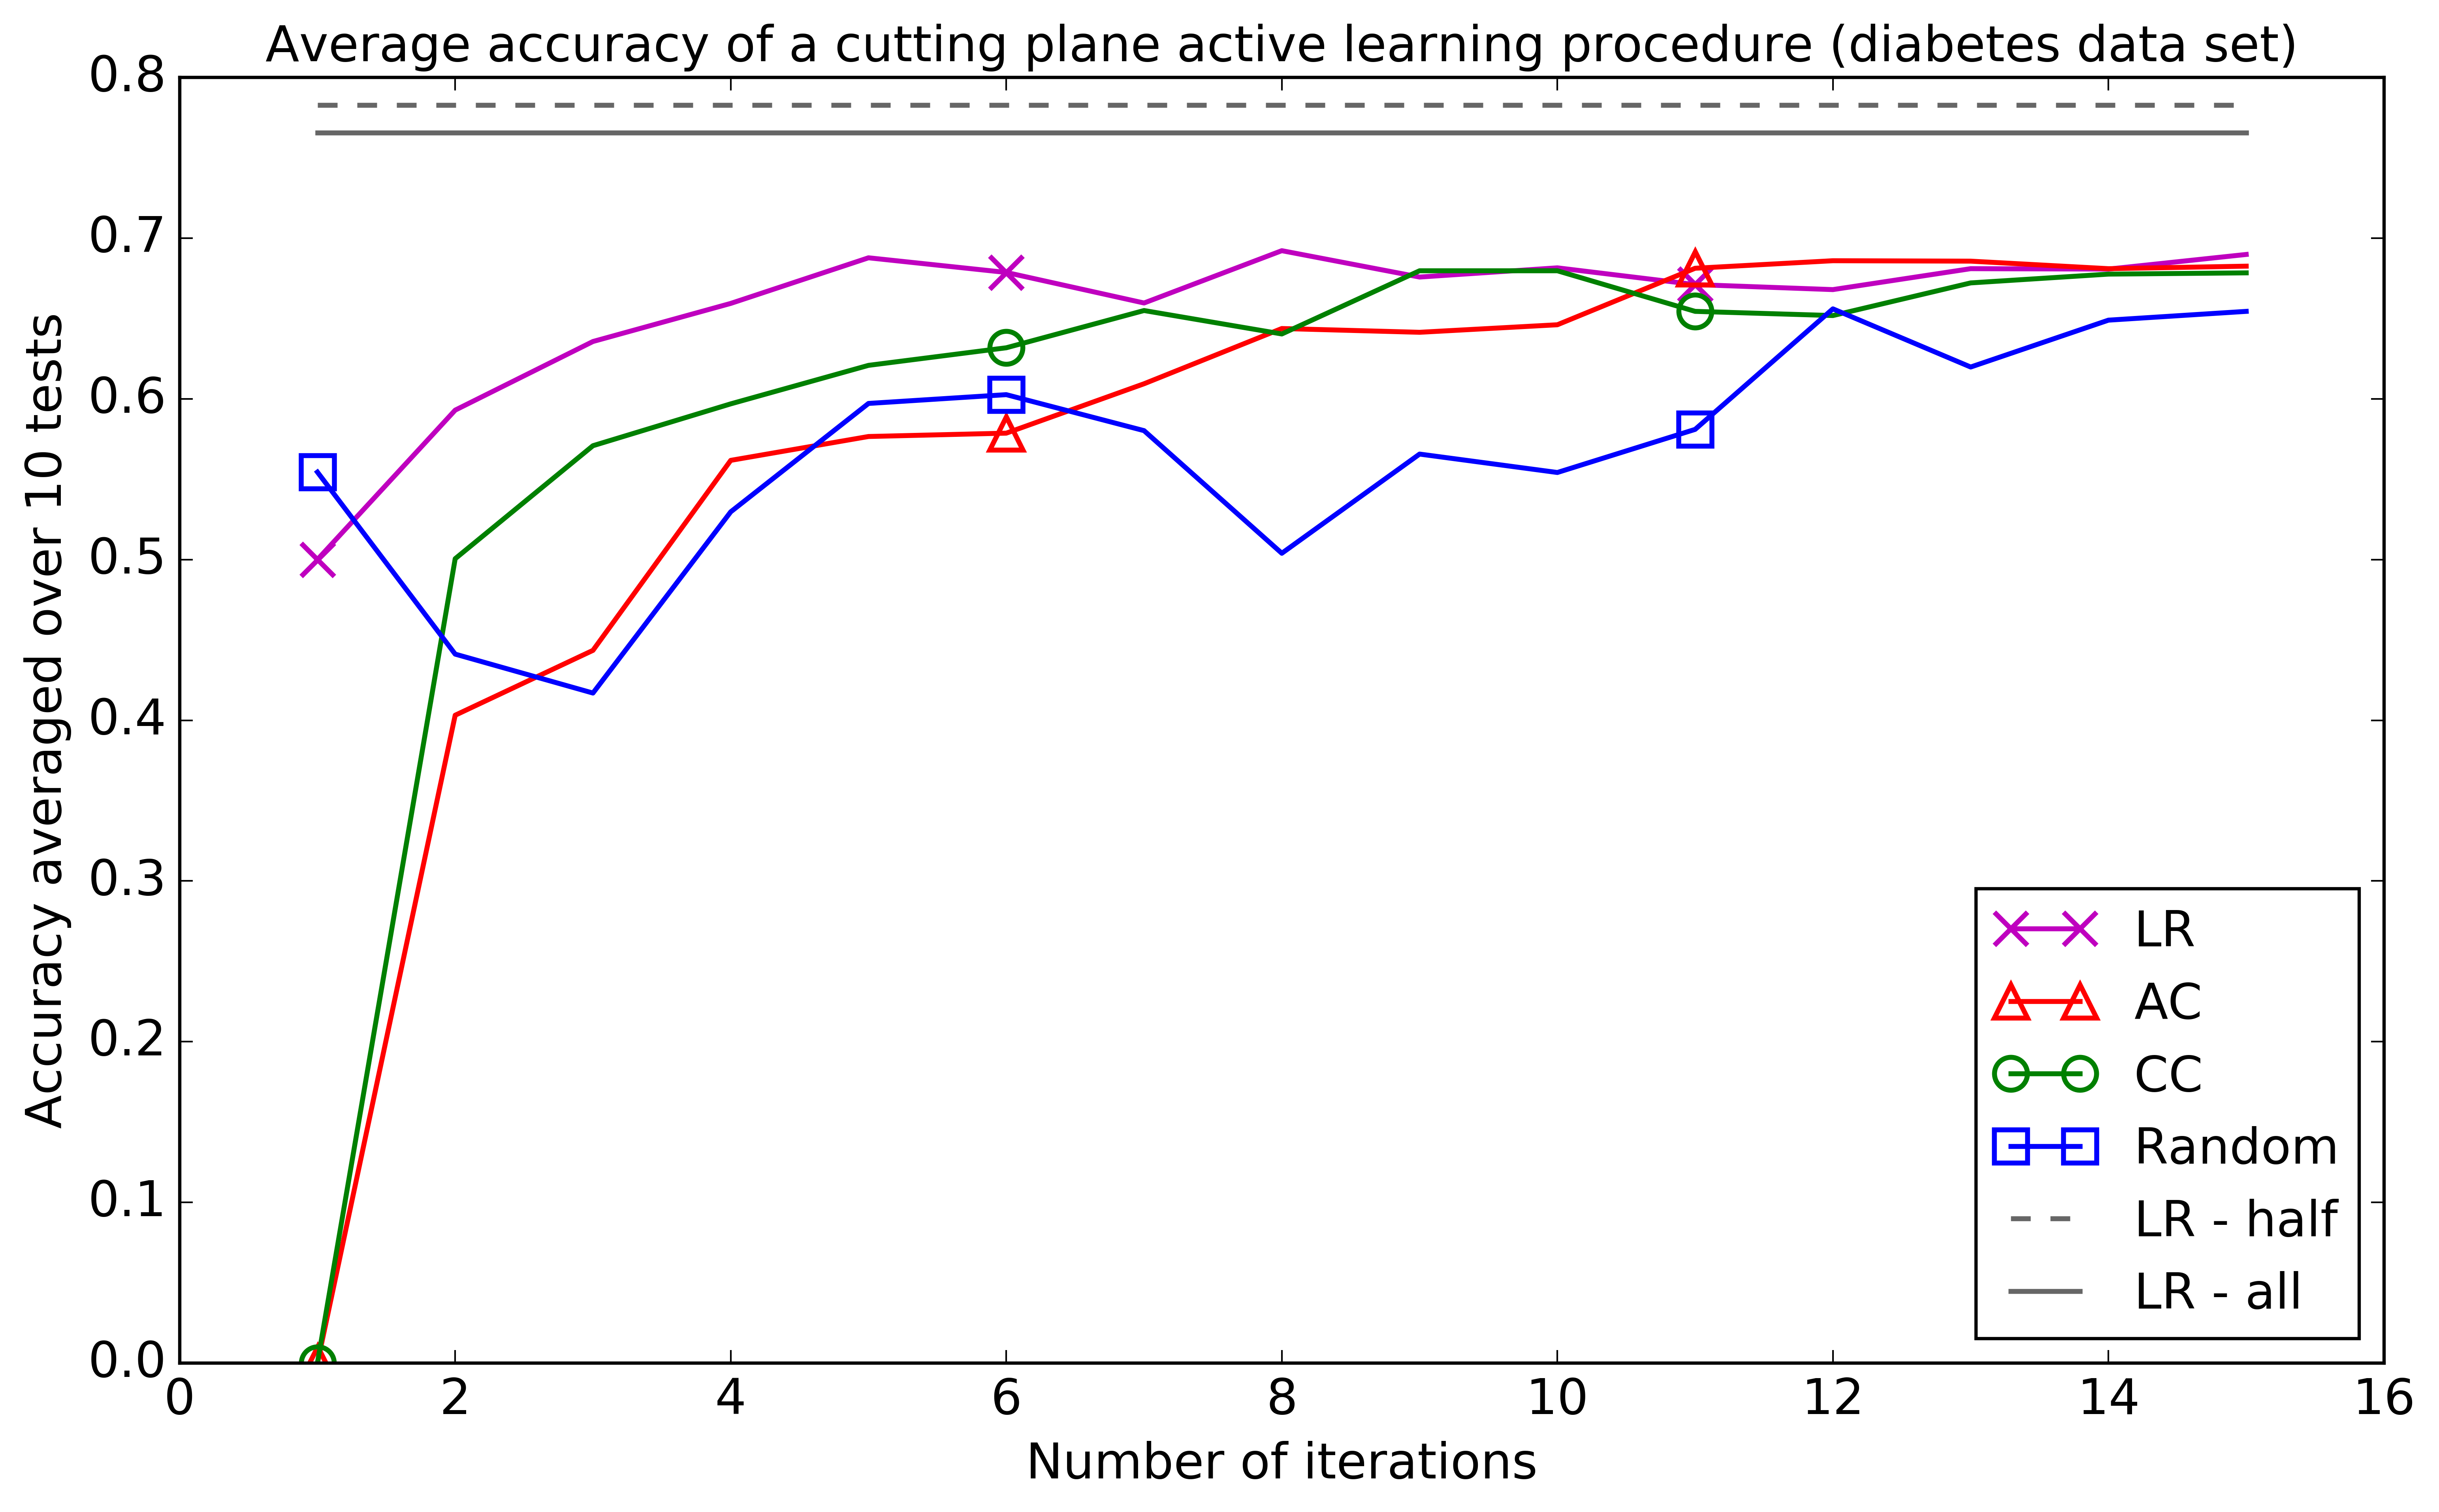
\includegraphics[width=\linewidth]{figures/diabetes_experiment.png}
        \end{figure}
\end{frame}

\begin{frame}{Conclusion}
      The general cutting-plane algorithm can be extended in a number of ways:
          \begin{enumerate}
        \item each iteration instead of returning a single cutting-plane, we can return \emph{ multiple} cutting-planes;
        \item each iteration we can remove (or in other words \emph{drop} or \emph{prune}) inequality constraints that may be redundant;
        \item we can limit the number of inequality constraints; and
        \item we can allow \emph{non-linear} cuts.
    \end{enumerate}

\end{frame}

\end{document}